\documentclass[11pt]{article}
\usepackage[margin=1.2in, top=0.5in, bottom=1in]{geometry}
\usepackage{graphicx}
\usepackage{parskip}
\usepackage[utf8]{inputenc}
\usepackage{hyperref}


\title{Algorithms for Speech and NLP --- TD 2 (NLP)}
\author{Hugo Cisneros}
\date{March 18th 2019}

\begin{document}
    \maketitle
    \section{System description}
    \begin{figure}[h]
        \centering
        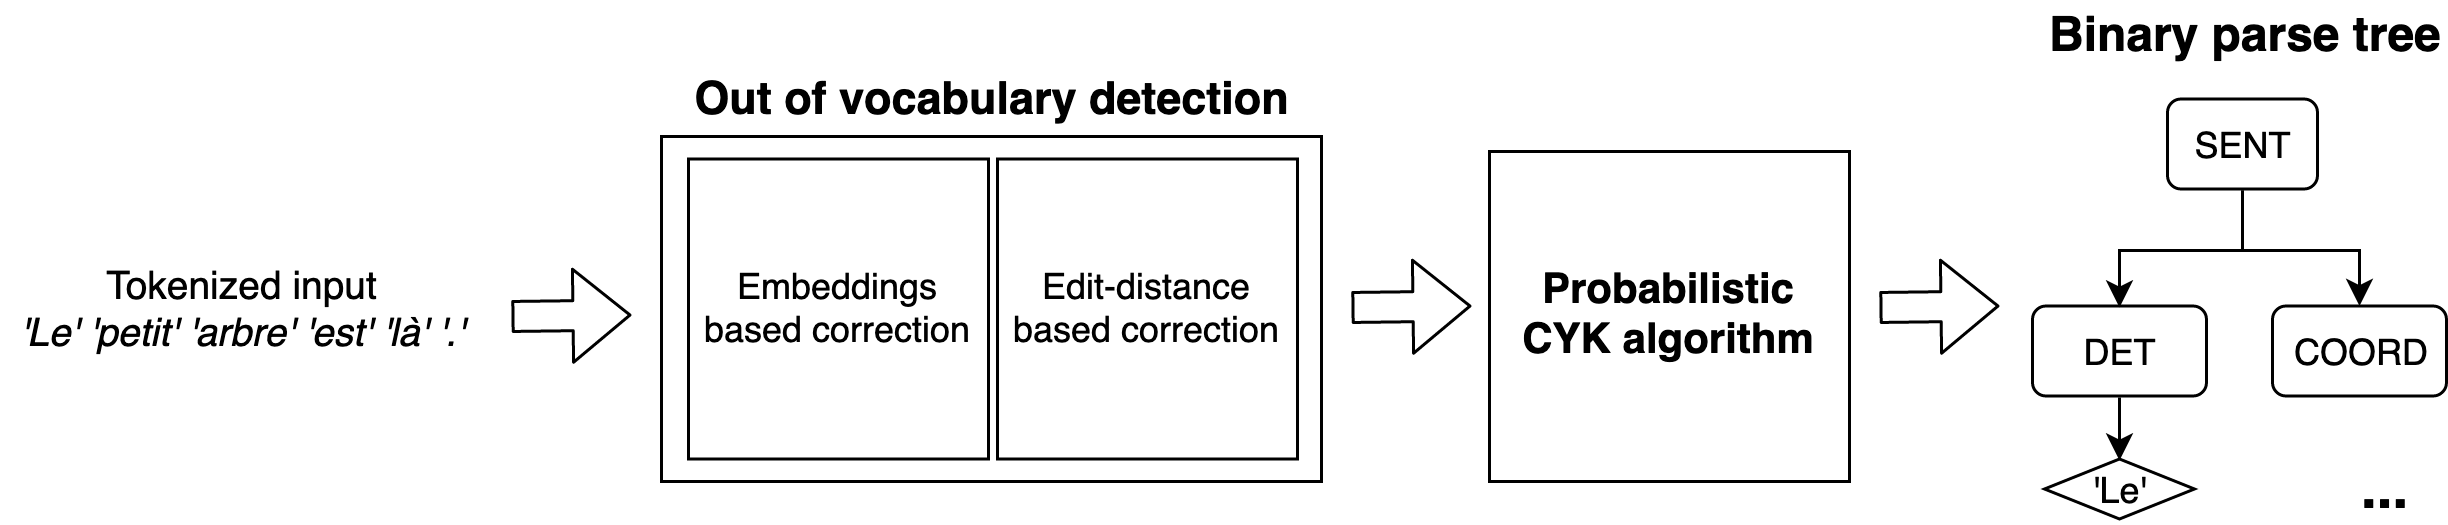
\includegraphics[width=.9\linewidth]{system.png}
        \caption{System overview}
        \label{fig:sys}
    \end{figure}
    The work I carried out for this project can be divided into two parts:
    \begin{itemize}
        \item Build a tree parsing system that can construct and save a PCFG 
        from a given treebank.
        \item Build the parser that uses the PCFG to parse input sentences. This 
        system is illustrated on Figure \ref{fig:sys} and is composed of an 
        a first part handling out-of-vocabulary (OOV) words by replacing them 
        with appropriate other words, and an implementation of the probabilistic
        CYK algorithm as described by Jurafsky and Martin in the draft of the 
        book \textit{Speech and Language Processing}
        \footnote{\url{https://web.stanford.edu/~jurafsky/slp3/}}
    \end{itemize}

    \subsection{PCFG building}
    The custom tree parsing system is based on detecting regular expressions and
    progressively substituting them to reduce the tree from bottom to top. 
    
    Example: \texttt{(SENT (NP (NPP Paul)) (V mange))} is first replaced by 
    \texttt{(SENT (NP (NPP)) (V))} and then \texttt{(SENT (NP) (V))} and finally
    \texttt{(SENT)}. At each step all elements substituted are added to the 
    grammar as rules.

    After, the grammar is transposed into Chomsky's normal form to be ready to
    use for the CYK algorithm. 

    \subsection{OOV substitution}
    OOV word substitution is done in two steps. If an unknown word exists in 
    the embedding dictionary (we used the French polyglot embeddings\footnote{
    \url{https://sites.google.com/site/rmyeid/projects/polyglot}}), the closest 
    (cosine distance wise) word from the lexicon is used as substitute. This 
    allows to replace words by others that have similar meaning and function in 
    a sentence.
    \begin{figure}[h]
        \centering
        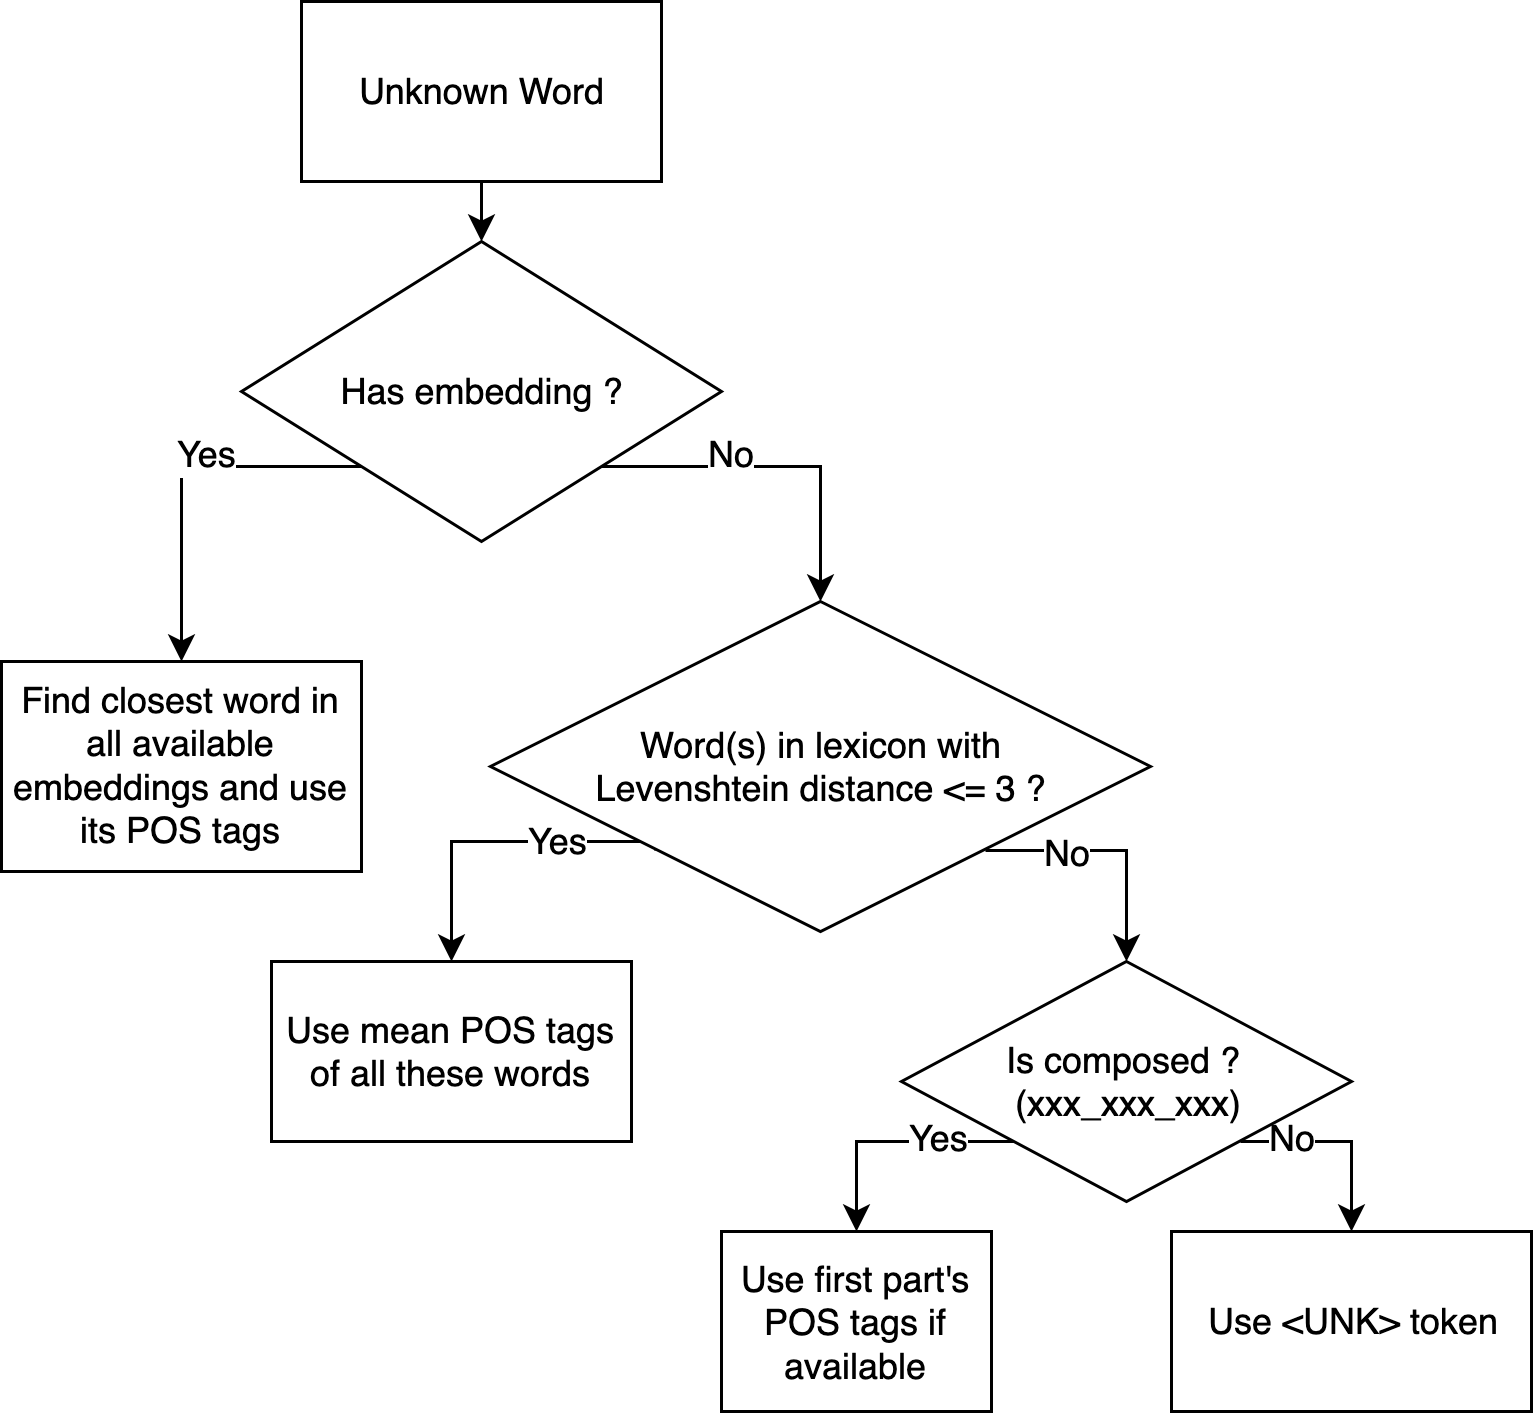
\includegraphics[width=.4\linewidth]{oov.png}
        \caption{OOV module overview}
        \label{fig:oov}
    \end{figure}

    In the cases where the word isn't in the embedding dictionary, is is 
    substituted with any word from the lexicon with levenshtein distance lower 
    than 2 from it. This allows to deal with small typos that are common in 
    user input. 

    For unknown group tokens of the form \texttt{xxxx\_xx\_xxx} that failed 
    the two first tests, the first part of the token \texttt{xxxx} is selected. 

    For other words, an \texttt{<UNK>} token mapping to all possible POS tags 
    with equal probability is used to make sure that completely unknown words 
    can still lead to a grammatically valid sentence. Figure \ref{fig:oov} 
    summarizes the whole system.

    \section{Error analysis}
    The resulting system sometimes cannot parse some sentences it consider 
    grammatically incorrect.
    The CYK algorithm is unable to correctly build the tree up to the start
    symbol. For 
    example, with the following sentence
    \texttt{Le juge d' Amiens se dessaisit du dossier.}, the token 
    \texttt{dessaisit} is replaced by \texttt{dessaisi} by the OOV module, 
    because it is only at a levenshtein distance of 1 from the original word. 
    However, the function of 
    this new word is radically different from the original one and the sentence
    \texttt{Le juge d' Amiens se dessaisi du dossier.} cannot lead to a 
    grammatically correct sentence when parsed with the CYK algorithm.

    Similarly, the sentence \texttt{Dans la maladie de Paget , le remodelage 
    osseux est trop \\rapide et l' os nouveau se forme de façon désordonnée , 
    ce qui le rend plus \\faible que l' os normal .} which has particularly 
    intricate structure, cannot be built from the learned grammar. 

    These two example are caused by sparsity issues with the model, and a 
    bigger training set of both words and sentences would help cope with these 
    problems.
\end{document}